% BÀI TOÁN HÌNH HỌC - BAI_HINH_13 (TRÍCH ĐỀ 13)
\begin{ex}
% Câu 13
Cho nửa đường tròn tâm $O$ đường kính $AB=2R$. Trên nửa mặt phẳng bờ $AB$, cùng phía với nửa đường tròn vẽ $Ax, By$ lần lượt là các tia tiếp tuyến của $(O)$ tại $A$ và $B$. Gọi $I$ là trung điểm của $AO$. Lấy hai điểm $P, Q$ nằm trên $Ax, By$ sao cho $\widehat{PIQ} = 90^\circ$. Gọi $H$ là hình chiếu vuông góc của $I$ lên $PQ$.
\begin{enumerate}
	\item Chứng minh tứ giác $APHI$ nội tiếp.
	\item Gọi $M, N$ lần lượt là giao điểm của $AH$ với $PI$ và $BH$ với $IQ$. Chứng minh $MN // AB$.
\end{enumerate}
\loigiai{
{
		\begin{center}
		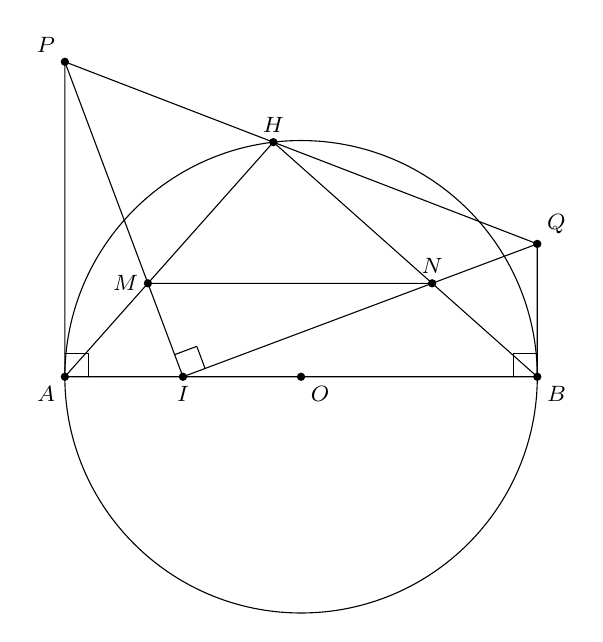
\begin{tikzpicture}[line join = round, line cap=round,>=stealth,font=\footnotesize,scale=1]
			\usetikzlibrary{calc,intersections,angles}
			
			% Khai báo hằng số
			\def\r{3} % r = 3cm
			\def\a{4} % a = 4
			
			% Định nghĩa tọa độ các điểm
			\coordinate (O) at (0,0);
			\coordinate (A) at (-\r,0);
			\coordinate (B) at (\r,0);
			\coordinate (I) at (-\r/2,0);
			\coordinate (P) at (-\r,\a);
			\coordinate (Q) at (\r,{3*\r^2/(4*\a)});
			
			% H là hình chiếu của I lên PQ
			\coordinate (H) at ($(P)!(I)!(Q)$);
			
			% M là giao điểm của AH và PI
			\path[name path=lineAH_M] (A) -- (H);
			\path[name path=linePI_M] (P) -- (I);
			\path[name intersections={of=lineAH_M and linePI_M, by=M}];
			
			% N là giao điểm của HB và IQ
			\path[name path=lineHB_N] (H) -- (B);
			\path[name path=lineIQ_N] (I) -- (Q);
			\path[name intersections={of=lineHB_N and lineIQ_N, by=N}];
			
			% Vẽ các đối tượng hình học
			\draw (O) circle (\r);          % Đường tròn (O;r)
			\draw (A) -- (B) -- (Q) -- (P) -- cycle; % Đa giác A-B-Q-P-A
			\draw (P) -- (I) -- (Q);        % Đường P-I-Q
			\draw (M) -- (N);               % Đoạn M-N
			\draw (A) -- (H) -- (B);        % Đường A-H-B
			
			% Tô màu cho các điểm (theo cấu trúc đầu tiên)
			\fill (O) circle (1.5pt);
			\fill (A) circle (1.5pt);
			\fill (B) circle (1.5pt);
			\fill (I) circle (1.5pt);
			\fill (P) circle (1.5pt);
			\fill (Q) circle (1.5pt);
			\fill (H) circle (1.5pt);
			\fill (M) circle (1.5pt);
			\fill (N) circle (1.5pt);
			
			% Đặt nhãn cho các điểm (theo cấu trúc đầu tiên)
			\node[below right] at (O) {$O$};
			\node[below left] at (A) {$A$};
			\node[below right] at (B) {$B$};
			\node[below] at (I) {$I$};
			\node[above left] at (P) {$P$};
			\node[above right] at (Q) {$Q$};
			\node[above] at (H) {$H$}; % Vị trí tương đối, có thể cần điều chỉnh
			\node[left] at (M) {$M$};   % Vị trí tương đối
			\node[above] at (N) {$N$};  % Vị trí tương đối
			
			% Ký hiệu các góc vuông
			% Góc PAO (vuông tại A)
			\pic[draw, angle radius=3mm]{right angle = P--A--O};
			% Góc QBA (vuông tại B)
			\pic[draw, angle radius=3mm]{right angle = Q--B--A};
			% Góc PIQ (vuông tại I)
			\pic[draw, angle radius=3mm]{right angle = P--I--Q}; % Tăng bán kính một chút cho dễ nhìn
			
		\end{tikzpicture}
		
		\end{center}
}
\end{ex}
